\documentclass[hyperref={pdfpagelabels=false}]{beamer}
\usepackage{lmodern}

\usetheme{Madrid}

\usepackage[slovak]{babel}
\usepackage[utf8]{inputenc}
\usepackage{amssymb,amsfonts,amscd}
\usepackage{times}
\usepackage[T1]{fontenc}
\usepackage{multirow}
\usepackage{wrapfig}
\usepackage{graphicx}

%\expandafter\def\expandafter\insertshorttitle\expandafter{%
%  \insertshorttitle\hfill%
%  \insertframenumber\,/\,\inserttotalframenumber}


\title[Teória hromadnej obsluhy]{Semestrálna práca "Supermarket"}
  
\author[Bc. Juraj Pobeha]{Bc. Juraj Pobeha}
 
\institute []
{  
  Žilinská Univerzita v Žiline\\
  Fakulta riadenia a informatiky
}

\date{15. decembra 2014} 
\begin{document}
\selectlanguage{slovak}

\begin{frame}
\titlepage
\end{frame} 


\begin{frame}
\frametitle{Obsah}
\tableofcontents
\end{frame} 


\section{Slovný popis úlohy} 
\begin{frame}
\frametitle{Slovný popis úlohy}
Modelujeme systém hromadnej obsluhy „Supermarket“. Do supermarketu prichádzajú zákazníci, ktorí sa po vybratí požadovaného tovaru presunú k pokladniam. V supermarkete sú 3 pokladne. Prvú obsluhuje skúsená (prioritná) predavačka , druhú novoprijatá (neprioritná) predavačka, ktorá sa ešte len zaúča a tretia pokladňa je samoobslužná. Zákazníci sa stavajú do jedného frontu, kde si vyberú obsluhu. S pravdepodobnosťou $\alpha$ si vyberú obsluhu skúsenou (prioritnou) predavačkou. Ak si vyberú obsluhu prioritnou predavačkou a tá je obsadená, presunú sa k neprioritnej. S pravdepodobnosťou $1-\alpha$ si vyberú obsluhu samoobslužnou pokladňou. Vstupný tok zákazníkov je elementárny s parametrom $\lambda$. Stredná doba obsluhy, či už u pokladníčok, alebo pri samoobslužnej pokladni má exponenciálne rozdelenie postupne s priemernými dobami $\frac{1}{\mu_1}$, $\frac{1}{\mu_2}$, $\frac{1}{\mu_3}$ .
\end{frame}

\begin{frame}
\frametitle{Grafické zobrazenie modelovaného systému}
\begin{figure}[!hlrbt]
\begin{center}
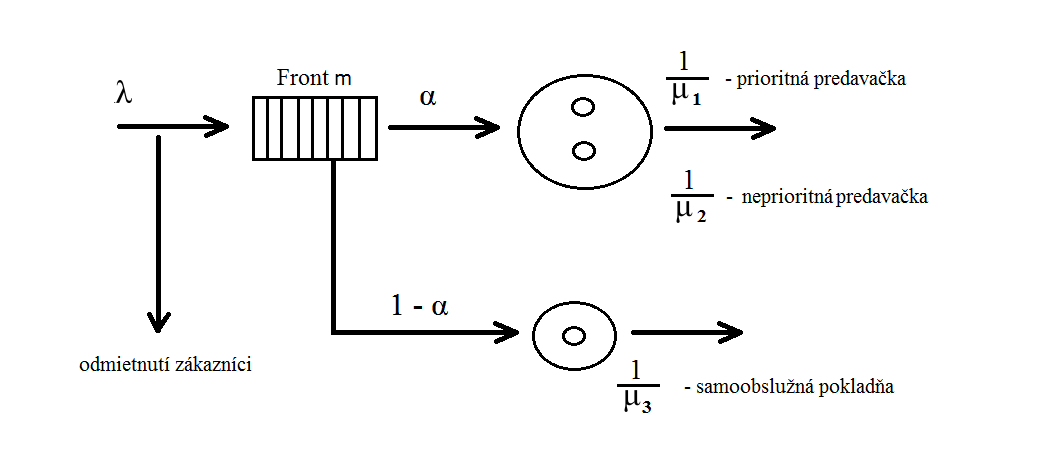
\includegraphics[width=13cm]{obrazky/supermarket1.png}
\end{center}
%\caption {kolmý priemet vektora {\bf f} do ''modrého'' a ''červeného'' podpriestoru}
\end{figure}
\end{frame}

\section{Popis stavov} 
\begin{frame}
\frametitle{Popis stavov v modelovanom systéme s konečným frontom dĺžky m = 3}
{\bf Vytvoríme maticu prechodov $Q = q_{ij}$} , pričom \\ 
\medskip
{\bf i} – počet zákazníkov vo fronte\\
{\bf i} $\in$ \{0, 1, 2, 3\}\\
\medskip
{\bf j} – stav obslužných liniek\\
{\bf j} $\in$ \{P, N, S, PN, PS, NS, PNS\}\\
\medskip
{\bf P} – obsluha prioritnou pokladňou\\
{\bf N} – obsluha neprioritnou pokladňou\\
{\bf S} – obsluha samoobslužnou pokladňou\\
\medskip
$\mathbb{S}$ - množina stavov\\
{\color{red} $\mathbb{S}$ = \{00, P0, N0, S0, PN0, PS0, NS0, PNS0, PNS1, PNS2, PNS3\}}\\
\medskip
{\bf 00} - prázdny systém\\
{\bf P0} - jeden zákazník obsluhovaný prioritnou pokladňou\\
{\bf PNS2} - všetky pokladne sú obsadené a 2 zákazníci čakajú vo fronte

\end{frame}

\begin{frame}
\frametitle{Prechodový graf}
\begin{figure}[!hlrbt]
\begin{center}
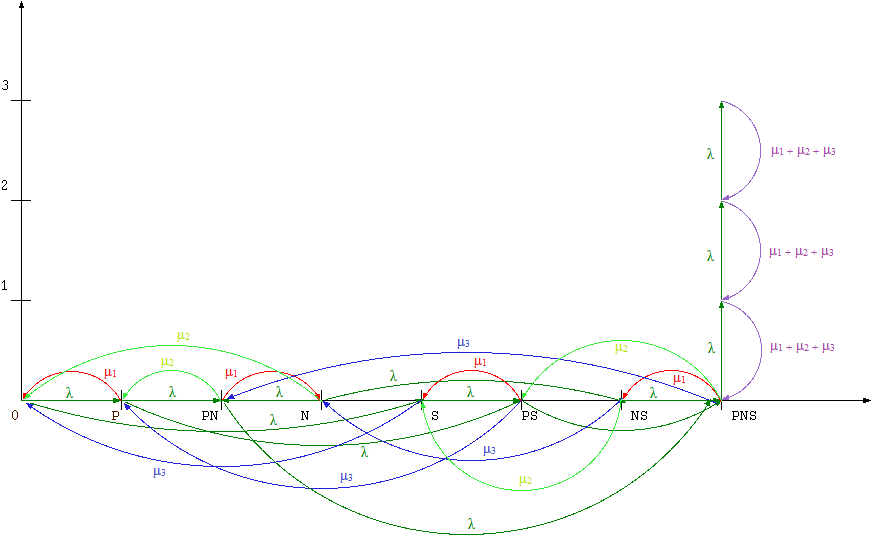
\includegraphics[width=12cm]{obrazky/graf.png}
\end{center}
\end{figure}
\end{frame}

\begin{frame}
\frametitle{Popis niektorých prechodov}
\begin{itemize}
\item Zo stavu 00 (prázdny systém) sa môžem dostať do stavu P0 (jeden zákazník obsluhovaný prioritnou pokladňou) s intenzitou $\alpha\lambda$ alebo do stavu S0 (jeden zákazník obsluhovaný samoobslužnou pokladňou s intenzitou (1-$\alpha)\lambda$. 
\item Zo stavu NS0 (obsluha neprioritnou a samoobslužnou pokladňou) sa môžem dostať do stavu PNS0 (všetky pokladne obsluhujú) s intenzitou $\alpha\lambda$, do stavu N0 (obsluha zákazníka neprioritnou pokladňou) s intenzitou $\mu_3$ a do stavu S0 (obsluha zákazníka samoobslužnou pokladňou) s intenzitou $\mu_2$. 
\item Do stavu PNS1 (všetky pokladne obsluhujú a jeden zákazník čaká vo fronte) sa môžem dostať iba zo stavu PNS0 (všetky pokladne obsluhujú). Zo stavu PNS1 sa môžem dostať iba do stavu PNS0 s intenzitou $\mu_1+\mu_2+\mu_3$.
\end{itemize}
\end{frame}

\section{Matica prechodov Q}
\begin{frame}
\frametitle{Matica prechodov Q}
\begin{figure}[!hlrbt]
\begin{center}
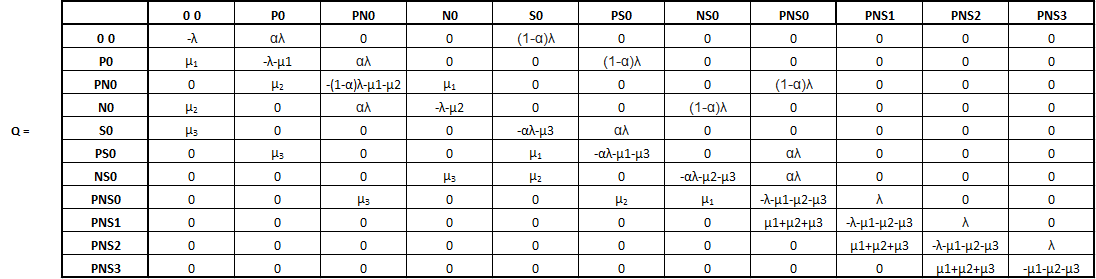
\includegraphics[width=12cm]{obrazky/maticaQ.png}
\end{center}
\end{figure}
\end{frame}

\section{Hľadanie stacionárneho rozdelenia}
\begin{frame}
\frametitle{Hľadanie stacionárneho rozdelenia pre $\alpha$=0}
\begin{figure}[!hlrbt]
\begin{center}
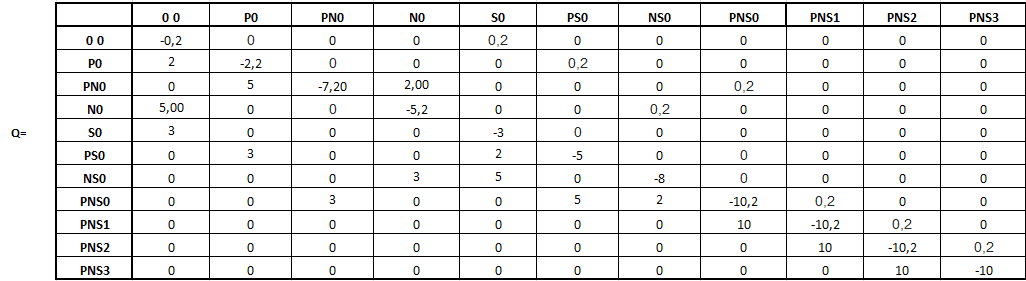
\includegraphics[width=12cm]{obrazky/maticaQ1.png}
\end{center}
\end{figure}
$\lambda$ = 0,2  (vstupný tok zákazníkov je 0,2 za minútu, čiže 12 zákazníkov za hodinu)\\
$\mu_1$ = 2 (stredná doba obsluhy prioritnej pokladne sú 2 minúty)\\
$\mu_2$ = 5 (stredná doba obsluhy neprioritnej pokladne je 5 minút)\\
$\mu_3$ = 3 (stredná doba obsluhy samoobslužnej pokladne sú 3 minúty)\\
$\alpha$ = 0 (pravdepodobnosť výberu obsluhy prioritnou pokladňou, ak je obsadená presun k neprioritnej)\\
1- $\alpha$ = 1 (pravdepodobnosť výberu obsluhy samoobslužnou pokladňou)
\end{frame}

\begin{frame}
\frametitle{Hľadanie stacionárneho rozdelenia  pre $\alpha$=0}
Keďže $\alpha$ = 0, vznikol nám jednolinkový systém hromadnej obsluhy.\\

\begin{figure}[!hlrbt]
\begin{center}
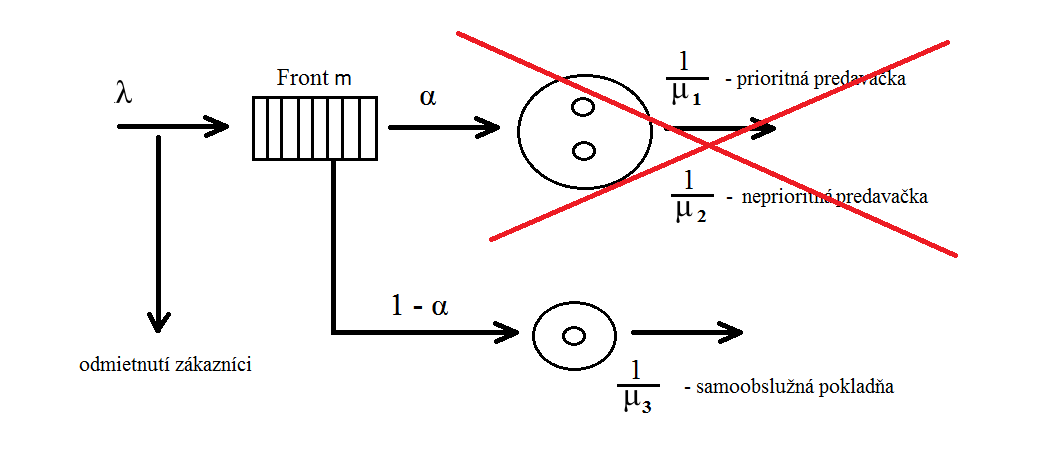
\includegraphics[width=12cm]{obrazky/supermarket2.png}
\end{center}
\end{figure}
\end{frame}

\begin{frame}
\frametitle{Hľadanie stacionárneho rozdelenia  pre $\alpha$=0}
V Markovovom procese určenom konečnou množinou stavov $\mathbb{S}$ a maticou intenzít {\bf Q} hľadáme stacionárne rozdelenie v tvare riešenia systému\\
\begin{center}
$\pi$ Q = 0, $\sum\limits_{j \in S}{} \pi_j$ = 1 , $\pi \geq$ 0\\
\end{center}
ktoré môžeme prepísať na tvar\\
\begin{center}
A$\pi^T = b^T, b = (0,0,...,0,1) \Rightarrow \pi^T = A^{-1} b^T$,
\end{center}
\end{frame}


\begin{frame}
\frametitle{Hľadanie stacionárneho rozdelenia  pre $\alpha$=0}
\begin{figure}[!hlrbt]
\begin{center}
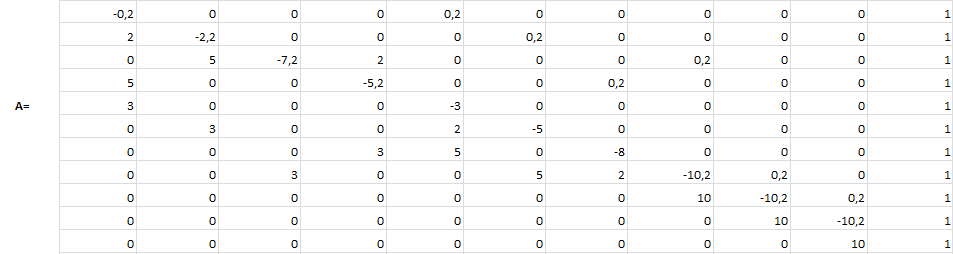
\includegraphics[width=12cm]{obrazky/maticaA.png}
\end{center}
\end{figure}
Posledný stĺpec matice A sme nahradili jednotkami.
\end{frame}

\begin{frame}
\frametitle{Hľadanie stacionárneho rozdelenia  pre $\alpha$=0}
\begin{figure}[!hlrbt]
\begin{center}
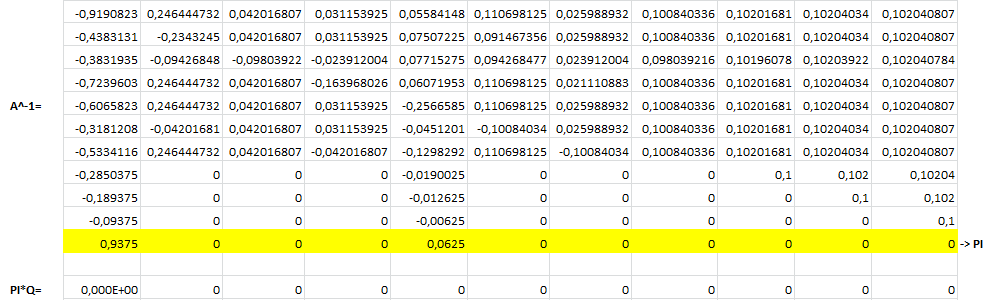
\includegraphics[width=12cm]{obrazky/maticaAmin1.png}
\end{center}
\end{figure}
$\pi$Q = 0 , našli sme stacionárne riešenie
\end{frame}


\begin{frame}
\frametitle{Hľadanie stacionárneho rozdelenia  pre $\alpha$=0}
Overenie riešenia:\\
Kostra\\

\begin{figure}[!hlrbt]
\begin{center}
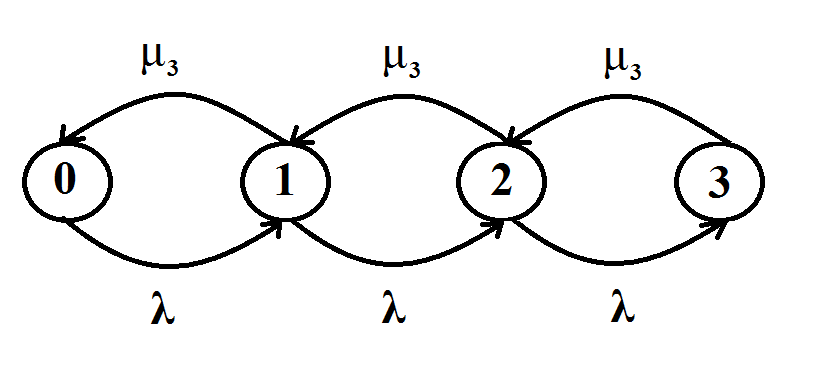
\includegraphics[width=9cm]{obrazky/kostra.png}
\end{center}
\end{figure}
$\pi_0=\frac{B_0}{B_0+B_1+B_2+B_3}$ , po dosadení $\pi_0$= 0,9333 $\doteq$ 0,9375 \\
$B_0=\mu_3^3$\\
$B_1=\lambda\mu_3^2$\\
$B_2=\lambda^2\mu_3$\\
$B_3=\lambda^3$
\end{frame}

\begin{frame}
\frametitle{Hľadanie stacionárneho rozdelenia pre $\alpha$=0.6, 1-$\alpha$=0.4}
$\alpha$ = 0,6 (pravdepodobnosť výberu obsluhy prioritnou pokladňou, ak je obsadená presun k neprioritnej)\\
1- $\alpha$ = 0,4 (pravdepodobnosť výberu obsluhy samoobslužnou pokladňou)
\begin{figure}[!hlrbt]
\begin{center}
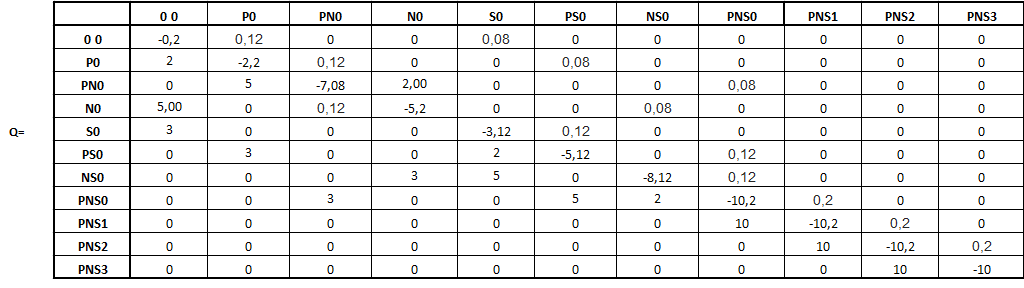
\includegraphics[width=12cm]{obrazky/maticaQ2.png}
\end{center}
\end{figure}
\end{frame}

\begin{frame}
\frametitle{Hľadanie stacionárneho rozdelenia pre $\alpha$=0.6, 1-$\alpha$=0.4}
\begin{figure}[!hlrbt]
\begin{center}
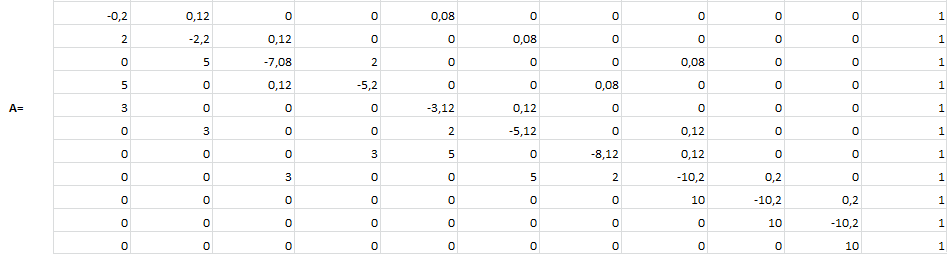
\includegraphics[width=12cm]{obrazky/maticaA2.png}
\end{center}
\end{figure}
Posledný stĺpec matice A sme nahradili jednotkami.
\end{frame}

\begin{frame}
\frametitle{Hľadanie stacionárneho rozdelenia pre $\alpha$=0.6, 1-$\alpha$=0.4}
\begin{figure}[!hlrbt]
\begin{center}
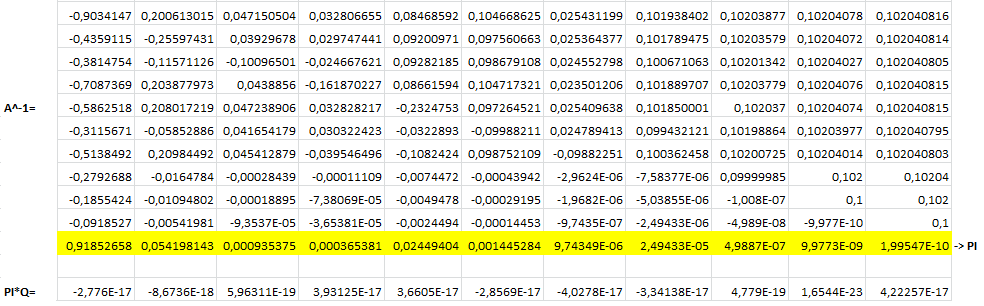
\includegraphics[width=12cm]{obrazky/maticaAmin2.png}
\end{center}
\end{figure}
$\pi$Q = 0, je to stacionárne riešenie
\end{frame}

\section{Optimalizačná úloha}
\begin{frame}
\frametitle{Optimalizačná úloha}
$c_p$ - mzda priorotnej predavačky v eurách na hodinu\\
$c_n$ - mzda neprioritnej predavačky v eurách na hodinu\\
$c_s$ - náklady na údržbu samoobslužnej pokladne v eurách na hodinu\\ 
$c_a$ - priemerná cena nákupu zákazníka v eurách\\
$c_r$ - jednotková cena za reklamu
\medskip \medskip

Cieľom optimalizačnej úlohy je nájsť takú intenzitu vstupného toku zákazníkov, pri ktorej bude zisk maximálny.\\

\medskip \medskip
Z($\lambda$) = $E(N_Q)c_a$ - $E(N_P)c_p$ - $E(N_N)c_n$ - $E(R_\lambda)c_r$

\medskip \medskip
$E(N_Q)c_a$ - priemerný príjem z obsluhy zákazníkov\\
$E(N_P)c_p$ - priemerné náklady na mzdu prioritnej predavačky podľa jej výkonnosti\\
$E(N_N)c_n$ - priemerné náklady na mzdu neprioritnej predavačky podľa jej výkonnosti\\
$E(R_\lambda)c_r$ - priemerné náklady vynaložené na reklamu
\end{frame}

\begin{frame}
\frametitle{Optimalizačná úloha}
$E(R_\lambda)$ je dané funkciou 0,4$\lambda$ - $\frac{\lambda^2}{3}$.\\
\medskip
Po dosadení príslušných hodnôt za $\lambda$ mi vyšli nasledovné funkčné hodnoty:
\begin{figure}[!hlrbt]
\begin{center}
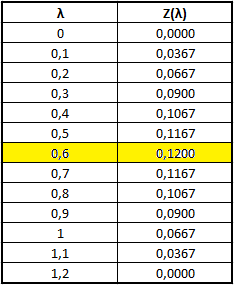
\includegraphics[width=4cm]{obrazky/opt.png}
\end{center}
\end{figure}
Najlepší výsledok vyšiel pre vstupný tok $\lambda$ = 0.6 zákazníkov za minútu (36 zákazníkov za hodinu).
\end{frame}

\begin{frame}
\frametitle{Optimalizačná úloha}
$E(R_\lambda)$ je dané funkciou 0,4$\lambda$ - $\frac{\lambda^2}{3}$.\\
\begin{figure}[!hlrbt]
\begin{center}
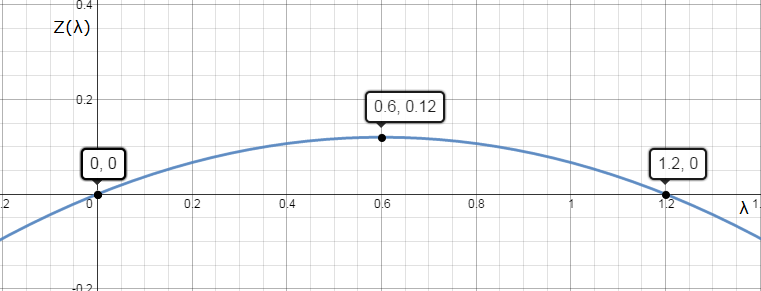
\includegraphics[width=12cm]{obrazky/opt1.png}
\end{center}
\end{figure}
\end{frame}

\section{Oblasti ďaľšieho skúmania}
\begin{frame}
\frametitle{Oblasti ďaľšieho skúmania}
\begin{itemize}
\item Zistiť optimálnu veľkosť nákladov na reklamu, aby sme prilákali čo najviac zákazníkov.
\medskip
\item Preskúmať, koľko pokladní by sme mali pridať, aby bol zisk z predaja čo najvyšší.
\end{itemize}
\end{frame}

\section{Záver}
\begin{frame}
\frametitle{Záver}
\begin{itemize}
\item V tejto semestrálnej práci som si precvičil základné poznatky z teórie hromadnej obsluhy nadobudnuté počas semestra.
\medskip
\item Riešil som systém hromadnej obsluhy "Supermarket", ktorý som popísal a následne spravil rôzne výpočty.
\medskip
\item Snažil som sa daný systém optimalizovať, čo sa mi čiastočne podarilo.
\end{itemize}
\end{frame}

\end{document}